%===============================================================================
% LaTeX sjabloon voor de bachelorproef toegepaste informatica aan HOGENT
% Meer info op https://github.com/HoGentTIN/latex-hogent-report
%===============================================================================

\documentclass[dutch,dit,thesis]{hogentreport}

% TODO:
% - If necessary, replace the option `dit`' with your own department!
%   Valid entries are dbo, dbt, dgz, dit, dlo, dog, dsa, soa
% - If you write your thesis in English (remark: only possible after getting
%   explicit approval!), remove the option "dutch," or replace with "english".

\usepackage{lipsum} % For blind text, can be removed after adding actual content

\usepackage[pdftex,bookmarks=true]{hyperref}
\usepackage[backend=biber,style=apa]{biblatex}

%% Pictures to include in the text can be put in the graphics/ folder
\graphicspath{{../graphics/}}

%% For source code highlighting, requires pygments to be installed
%% Compile with the -shell-escape flag!
%% \usepackage[chapter]{minted}
%% If you compile with the make_thesis.{bat,sh} script, use the following
%% import instead:
\usepackage[chapter,outputdir=../output]{minted}
\usemintedstyle{solarized-light}

%% Formatting for minted environments.
\setminted{%
    autogobble,
    frame=lines,
    breaklines,
    linenos,
    tabsize=4
}

%% Ensure the list of listings is in the table of contents
\renewcommand\listoflistingscaption{%
    \IfLanguageName{dutch}{Lijst van codefragmenten}{List of listings}
}
\renewcommand\listingscaption{%
    \IfLanguageName{dutch}{Codefragment}{Listing}
}
\renewcommand*\listoflistings{%
    \cleardoublepage\phantomsection\addcontentsline{toc}{chapter}{\listoflistingscaption}%
    \listof{listing}{\listoflistingscaption}%
}

% Other packages not already included can be imported here

%%---------- Document metadata -------------------------------------------------
% TODO: Replace this with your own information
\author{Brecht Roosens}
\supervisor{Dhr. S. De Gheselle}
\cosupervisor{Dhr. B. Rogge}
\title[Optionele ondertitel]%
    {Met Machine Learning een voorspellend onderhoudsmodel maken voor bouwmachines in kleine bouwondernemingen}
\academicyear{\advance\year by -1 \the\year--\advance\year by 1 \the\year}
\examperiod{1}
\degreesought{\IfLanguageName{dutch}{Professionele bachelor in de toegepaste informatica}{Bachelor of applied computer science}}
\partialthesis{false} %% To display 'in partial fulfilment'
%\institution{Internshipcompany BVBA.}

%% Add global exceptions to the hyphenation here
\hyphenation{back-slash}

%% The bibliography (style and settings are  found in hogentthesis.cls)
\addbibresource{bachproef.bib}            %% Bibliography file
\addbibresource{../voorstel/voorstel.bib} %% Bibliography research proposal
\defbibheading{bibempty}{}

%% Prevent empty pages for right-handed chapter starts in twoside mode
\renewcommand{\cleardoublepage}{\clearpage}

\renewcommand{\arraystretch}{1.2}

%% Content starts here.
\begin{document}

%---------- Front matter -------------------------------------------------------

\frontmatter

\hypersetup{pageanchor=false} %% Disable page numbering references
%% Render a Dutch outer title page if the main language is English
\IfLanguageName{english}{%
    %% If necessary, information can be changed here
    \degreesought{Professionele Bachelor toegepaste informatica}%
    \begin{otherlanguage}{dutch}%
       \maketitle%
    \end{otherlanguage}%
}{}

%% Generates title page content
\maketitle
\hypersetup{pageanchor=true}

%%=============================================================================
%% Voorwoord
%%=============================================================================

\chapter*{\IfLanguageName{dutch}{Woord vooraf}{Preface}}%
\label{ch:voorwoord}

%% TODO:
%% Het voorwoord is het enige deel van de bachelorproef waar je vanuit je
%% eigen standpunt (``ik-vorm'') mag schrijven. Je kan hier bv. motiveren
%% waarom jij het onderwerp wil bespreken.
%% Vergeet ook niet te bedanken wie je geholpen/gesteund/... heeft

Het probleem dat ik gekozen is gebaseerd op mijn bevindingen tijdens mijn studentenjob in de bouw. Mijn studentenjob heb ik gedaan via het bedrijf waar mijn vader en nonkel werken, namelijk Bouwonderneming Marchand BV, ik heb daar veel manuele taken uitgevoerd. Maar mijn idee is ontstaan door het probleem dat wil voorkwam op de werf waar ik meewerkte waar dikwijls de kraan eens een defect had of de kraan van de vraachtwagen eens niet werkte door een slecht contact in de elektriciteitbekabeling van de kraan. Door kwam ik op het idee om een voorspellend onderhoudsmodel te maken met unsupervised learning om daardoor defecten, storingen en piekende of dalende parameters te detecteren en daardoor te kosten van stilstand, kapotte onderdelen en onderhoud aan de machines te vervroegen. Hierdoor kunnen we kosten en tijd besparen door op voorhand te weten te komen wat er gaande is in de machine. Later verder aanvullen...
%%=============================================================================
%% Samenvatting
%%=============================================================================

% TODO: De "abstract" of samenvatting is een kernachtige (~ 1 blz. voor een
% thesis) synthese van het document.
%
% Een goede abstract biedt een kernachtig antwoord op volgende vragen:
%
% 1. Waarover gaat de bachelorproef?
% 2. Waarom heb je er over geschreven?
% 3. Hoe heb je het onderzoek uitgevoerd?
% 4. Wat waren de resultaten? Wat blijkt uit je onderzoek?
% 5. Wat betekenen je resultaten? Wat is de relevantie voor het werkveld?
%
% Daarom bestaat een abstract uit volgende componenten:
%
% - inleiding + kaderen thema
% - probleemstelling
% - (centrale) onderzoeksvraag
% - onderzoeksdoelstelling
% - methodologie
% - resultaten (beperk tot de belangrijkste, relevant voor de onderzoeksvraag)
% - conclusies, aanbevelingen, beperkingen
%
% LET OP! Een samenvatting is GEEN voorwoord!

%%---------- Nederlandse samenvatting -----------------------------------------
%
% TODO: Als je je bachelorproef in het Engels schrijft, moet je eerst een
% Nederlandse samenvatting invoegen. Haal daarvoor onderstaande code uit
% commentaar.
% Wie zijn bachelorproef in het Nederlands schrijft, kan dit negeren, de inhoud
% wordt niet in het document ingevoegd.

\IfLanguageName{english}{%
\selectlanguage{dutch}
\chapter*{Samenvatting}
\selectlanguage{english}
}{}

%%---------- Samenvatting -----------------------------------------------------
% De samenvatting in de hoofdtaal van het document

\chapter*{\IfLanguageName{dutch}{Samenvatting}{Abstract}}

Onvoorziene defecten van bouwmachines kunnen resulteren in stilstand, vertragingen en extra onderhoudskosten. Voorspellend onderhoud creëert kansen om afwijkend machinegedrag op tijd te waarnemen en onderhoud effectiever te organiseren. Voor kleine bouwbedrijven kan dit echter een uitdaging zijn, omdat er vaak slechts een beperkte hoeveelheid historische sensordata en een beperkt aantal geregistreerde defecten beschikbaar is. Deze bachelorproef bestudeert hoe een machine learning-methodiek, die steunt op sensordata, kan worden ingezet om storingen in bouwmachines in een kleine bouwbedrijf te voorspellen en het onderhoud efficiënter te plannen.

Voor het onderzoek zijn real-world telematicadata van een tractor die wordt ingezet voor grondverzet en transport gebruikt. Eerst werden de data opgeslagen, samengevoegd en voorbereid als een tijdsreeksdataset. Daarna werden belangrijke sensoren gekozen die informatie verstrekken over onder andere temperatuur, druk, motorbelasting, motortoerental en brandstofverbruik. Omdat de private tractordataset geen duidelijke defect- of onderhoudslabels had, werd er extra gebruikgemaakt van de openbare MetroPT-3-dataset. Deze dataset omvat industriële tijdsreeksdata met vastgelegde defectmomenten, waardoor het mogelijk werd  om de ontwikkelde methodiek objectiever te beoordelen.

In de methodiek zijn vijf modellen bestudeerd: Random Forest-model, Isolation Forest-model, Autoencoder, LSTM Autoencoder en One-Class SVM-model. De modellen werden aanvankelijk gebruikt op de MetroPT-3-dataset en daarna, waar mogelijk, op de private tractordataset. De uitkomsten gaven aan dat de prestaties aanzienlijk afhankelijk zijn van de gekozen methode en evaluatiemaatstaf. De Autoencoder leverde de beste resultaten op voor de defectklasse tijdens de aangepaste MetroPT-3-testperiode met een recall van 0.44 en een F1-score van 0.24. Random Forest-model en Isolation Forest-model ontdekten slechts een klein aantal van de geregistreerde defecten, terwijl One-Class SVM-model meer defecten kon opsporen, maar tegelijkertijd veel gebruikelijke observaties als een anomalie beschouwde.

Het onderzoek laat zien dat machine learning kan worden gebruikt om afwijkend gedrag in industriële sensordata te identificeren, wat een fundament kan leggen voor voorspellend onderhoud van bouwmachines. De implementatie van de private tractordataset heeft aangetoond dat de methodiek ook toepasbaar is voor real-world sensorgegevens, maar dat de ontdekte afwijkingen door het ontbreken van defectlabels niet als bevestigde storingen kunnen worden gezien. De ontwikkelde methode fungeert daarom voornamelijk als een bewijs. Voor een betrouwbare praktijktoepassing zijn uitgebreide historische datasets,  verschillende onderhouds- en storingsmomenten vereist. Dit maakt het mogelijk om toekomstige modellen effectiever te valideren en verder te optimaliseren voor gebruik in kleine bouwbedrijven.

%Onvoorziene defecten van bouwmachines kunnen resulteren in stilstand, vertragingen en extra onderhoudskosten. Voor kleine bouwbedrijven biedt voorspellend onderhoud een boeiende kans om machineproblemen vroegtijdig te herkennen en het onderhoud effectiever te plannen. In de praktijk hebben dergelijke bedrijven vaak een beperkte hoeveelheid historische sensordata en zijn er weinig of geen geregistreerde defecten. Dit maakt het niet vanzelfsprekend om traditionele machine learning-modellen voor het voorspellen van storingen direct in te zetten. Deze bachelorproef bestudeert hoe een machine learning-methodiek, die steunt op sensordata, kan worden ingezet om storingen in bouwmachines in een kleine bouwbedrijf te voorspellen en het onderhoud efficiënter te plannen.

%Het onderzoek vond plaats in samenwerking met een kleine bouwbedrijf en gebruikte real-world telematicadata van een tractor die wordt gebruikt voor grondverzet en transport. Eerst werden de beschikbare data opgeslagen en voorbereid voor een verdere analyse. Onder andere zijn er diverse databestanden samengevoegd, zijn tijdstempels gestandaardiseerd, zijn onnodige data verwijderd en zijn sensordata omgezet naar de juiste numerieke waarden. Daarna werden belangrijke parameters gekozen die informatie verstrekken over onder andere motorbelasting, temperatuur, druk, motortoerental en brandstofverbruik.

%Een cruciale beperking van de private tractordataset was het gebrek aan heldere historische defect- en onderhoudslabels. Hierdoor was het niet mogelijk om direct vast te stellen of een gedetecteerde afwijking overeenkwam met een echte machinefout. Om de ontwikkelde methodiek op een dataset met bekende tekortkomingen te kunnen beoordelen, werd er extra gebruikgemaakt van de openbare MetroPT-3-dataset. Deze dataset omvat tijdsreeksgegevens van een industrieel compressorsysteem en registreert defectmomenten. hierdoor was het mogelijk om de effectiviteit van de diverse methoden te evalueren op basis van bekende afwijkingen.







%---------- Inhoud, lijst figuren, ... -----------------------------------------

\tableofcontents

% In a list of figures, the complete caption will be included. To prevent this,
% ALWAYS add a short description in the caption!
%
%  \caption[short description]{elaborate description}
%
% If you do, only the short description will be used in the list of figures

\listoffigures

% If you included tables and/or source code listings, uncomment the appropriate
% lines.
\listoftables

\listoflistings

% Als je een lijst van afkortingen of termen wil toevoegen, dan hoort die
% hier thuis. Gebruik bijvoorbeeld de ``glossaries'' package.
% https://www.overleaf.com/learn/latex/Glossaries

%---------- Kern ---------------------------------------------------------------

\mainmatter{}

% De eerste hoofdstukken van een bachelorproef zijn meestal een inleiding op
% het onderwerp, literatuurstudie en verantwoording methodologie.
% Aarzel niet om een meer beschrijvende titel aan deze hoofdstukken te geven of
% om bijvoorbeeld de inleiding en/of stand van zaken over meerdere hoofdstukken
% te verspreiden!

%%=============================================================================
%% Inleiding
%%=============================================================================

\chapter{\IfLanguageName{dutch}{Inleiding}{Introduction}}%
\label{ch:inleiding}

%De inleiding moet de lezer net genoeg informatie verschaffen om het onderwerp te begrijpen en in te zien waarom de onderzoeksvraag de moeite waard is om te onderzoeken. In de inleiding ga je literatuurverwijzingen beperken, zodat de tekst vlot leesbaar blijft. Je kan de inleiding verder onderverdelen in secties als dit de tekst verduidelijkt. Zaken die aan bod kunnen komen in de inleiding~\autocite{Pollefliet2011}:

%\begin{itemize}
  %\item context, achtergrond
  %\item afbakenen van het onderwerp
  %\item verantwoording van het onderwerp, methodologie
  %\item probleemstelling
  %\item onderzoeksdoelstelling
  %\item onderzoeksvraag
  %\item \ldots
%\end{itemize}

\section{\IfLanguageName{dutch}{Probleemstelling}{Problem Statement}}%
\label{sec:probleemstelling}

%Uit je probleemstelling moet duidelijk zijn dat je onderzoek een meerwaarde heeft voor een concrete doelgroep. De doelgroep moet goed gedefinieerd en afgelijnd zijn. Doelgroepen als ``bedrijven,'' ``KMO's'', systeembeheerders, enz.~zijn nog te vaag. Als je een lijstje kan maken van de personen/organisaties die een meerwaarde zullen vinden in deze bachelorproef (dit is eigenlijk je steekproefkader), dan is dat een indicatie dat de doelgroep goed gedefinieerd is. Dit kan een enkel bedrijf zijn of zelfs één persoon (je co-promotor/opdrachtgever).%/

Graafmachines, hijskranen en betonpompen zijn cruciaal voor de dagelijkse activiteiten van kleine bouwbedrijven en hebben een directe impact op zowel de productiviteit als de kosten van
een bouwproject waaraan het bedrijf werkt \autocite{Mikulic2024}. Als deze machines plotseling defect raken, resulteert dit vaak in stilstand, vertragingen en aanzienlijke kosten voor reparaties van de machines \autocite{ErRatby2025}. In tal van kleine bouwondernemingen wordt onderhoud tegenwoordig nog altijd voornamelijk preventief uitgevoerd op vaste tijdstippen. Volgens
het onderzoek van \textcite{Morganti2024} en \textcite{Deepak2025} tonen zij aan dat deze methode niet altijd effectief is en dit kan resulteren in onnodige onderhoudskosten of onvoorziene stilstanden van de machines.

\section{\IfLanguageName{dutch}{Onderzoeksvraag}{Research question}}%
\label{sec:onderzoeksvraag}

%Wees zo concreet mogelijk bij het formuleren van je onderzoeksvraag. Een onderzoeksvraag is trouwens iets waar nog niemand op dit moment een antwoord heeft (voor zover je kan nagaan). Het opzoeken van bestaande informatie (bv. ``welke tools bestaan er voor deze toepassing?'') is dus geen onderzoeksvraag. Je kan de onderzoeksvraag verder specifiëren in deelvragen. Bv.~als je onderzoek gaat over performantiemetingen, dan 

De belangrijkste onderzoeksvraag is: Op welke manier kan een machine learningmodel, gebaseeerd op sensorgegevens, worden gebruikt om storingen in bouwmachines bij een kleine bouwonderneming nauwkeurig te voorspellen en het onderhoud effectiever te organiseren?
Eerst wordt onderzocht welke soorten sensordata en onderhoudsproblemen van belang zijn voor bouwmachines \autocite{Mikulic2024, Nayak2024}. Welke technische beperkingen er zijn binnen kleine bouwondernemingen \autocite{Elahi2023}. 
Zoals \textcite{Carvalho2019}, \textcite{Roehrich2024}, \textcite{Li2025} en \textcite{Wang2025} ook in hun onderzoek beschrijven, kan daarna pas onderzocht worden welke machine learning algoritmes geschikt zijn voor voorspellend onderhoud en op welke manier deze correct kunnen worden beoordeeld.

\section{\IfLanguageName{dutch}{Onderzoeksdoelstelling}{Research objective}}%
\label{sec:onderzoeksdoelstelling}

%Wat is het beoogde resultaat van je bachelorproef? Wat zijn de criteria voor succes? Beschrijf die zo concreet mogelijk. Gaat het bv.\ om een proof-of-concept, een prototype, een verslag met aanbevelingen, een vergelijkende studie, enz.

Deze bachelorproef heeft als doel een soort van proof-of-concept voorspellend onderhoudsmodel te creëren en te evalueren voor de gekozen casus. Dit wordt ook aangevuld met een praktisch
adviesrapport om het model te integreren en uit te voeren binnen het bedrijf. De bachelorproef is pas succesvol, zoals \textcite{Raffaele2024} en \textcite{Mahale2025} ook beschrijven in hun onderzoek, als het model technisch helemaal goed functioneert en een duidelijke waarde toevoegt aan het onderhoudsbeleid van het bouwbedrijf.

\section{\IfLanguageName{dutch}{Opzet van deze bachelorproef}{Structure of this bachelor thesis}}%
\label{sec:opzet-bachelorproef}

% Het is gebruikelijk aan het einde van de inleiding een overzicht te
% geven van de opbouw van de rest van de tekst. Deze sectie bevat al een aanzet
% die je kan aanvullen/aanpassen in functie van je eigen tekst.

De rest van deze bachelorproef is als volgt opgebouwd:

In Hoofdstuk~\ref{ch:stand-van-zaken} wordt een overzicht gegeven van de stand van zaken binnen het onderzoeksdomein, op basis van een literatuurstudie.

In Hoofdstuk~\ref{ch:methodologie} wordt de methodologie toegelicht en worden de gebruikte onderzoekstechnieken besproken om een antwoord te kunnen formuleren op de onderzoeksvragen.

% TODO: Vul hier aan voor je eigen hoofstukken, één of twee zinnen per hoofdstuk

In Hoofdstuk~\ref{ch:conclusie}, tenslotte, wordt de conclusie gegeven en een antwoord geformuleerd op de onderzoeksvragen. Daarbij wordt ook een aanzet gegeven voor toekomstig onderzoek binnen dit domein.
\chapter{\IfLanguageName{dutch}{Stand van zaken}{State of the art}}%
\label{ch:stand-van-zaken}

% Tip: Begin elk hoofdstuk met een paragraaf inleiding die beschrijft hoe
% dit hoofdstuk past binnen het geheel van de bachelorproef. Geef in het
% bijzonder aan wat de link is met het vorige en volgende hoofdstuk.

% Pas na deze inleidende paragraaf komt de eerste sectiehoofding.

%Dit hoofdstuk bevat je literatuurstudie. De inhoud gaat verder op de inleiding, maar zal het onderwerp van de bachelorproef *diepgaand* uitspitten. De bedoeling is dat de lezer na lezing van dit hoofdstuk helemaal op de hoogte is van de huidige stand van zaken (state-of-the-art) in het onderzoeksdomein. Iemand die niet vertrouwd is met het onderwerp, weet nu voldoende om de rest van het verhaal te kunnen volgen, zonder dat die er nog andere informatie moet over opzoeken \autocite{Pollefliet2011}.

%Je verwijst bij elke bewering die je doet, vakterm die je introduceert, enz.\ naar je bronnen. In \LaTeX{} kan dat met het commando \texttt{$\backslash${textcite\{\}}} of \texttt{$\backslash${autocite\{\}}}. Als argument van het commando geef je de ``sleutel'' van een ``record'' in een bibliografische databank in het Bib\LaTeX{}-formaat (een tekstbestand). Als je expliciet naar de auteur verwijst in de zin (narratieve referentie), gebruik je \texttt{$\backslash${}textcite\{\}}. Soms is de auteursnaam niet expliciet een onderdeel van de zin, dan gebruik je \texttt{$\backslash${}autocite\{\}} (referentie tussen haakjes). Dit gebruik je bv.~bij een citaat, of om in het bijschrift van een overgenomen afbeelding, broncode, tabel, enz. te verwijzen naar de bron. In de volgende paragraaf een voorbeeld van elk.

%\textcite{Knuth1998} schreef een van de standaardwerken over sorteer- en zoekalgoritmen. Experten zijn het erover eens dat cloud computing een interessante opportuniteit vormen, zowel voor gebruikers als voor dienstverleners op vlak van informatietechnologie~\autocite{Creeger2009}.

%Let er ook op: het \texttt{cite}-commando voor de punt, dus binnen de zin. Je verwijst meteen naar een bron in de eerste zin die erop gebaseerd is, dus niet pas op het einde van een paragraaf.

%\begin{figure}
  %\centering
  %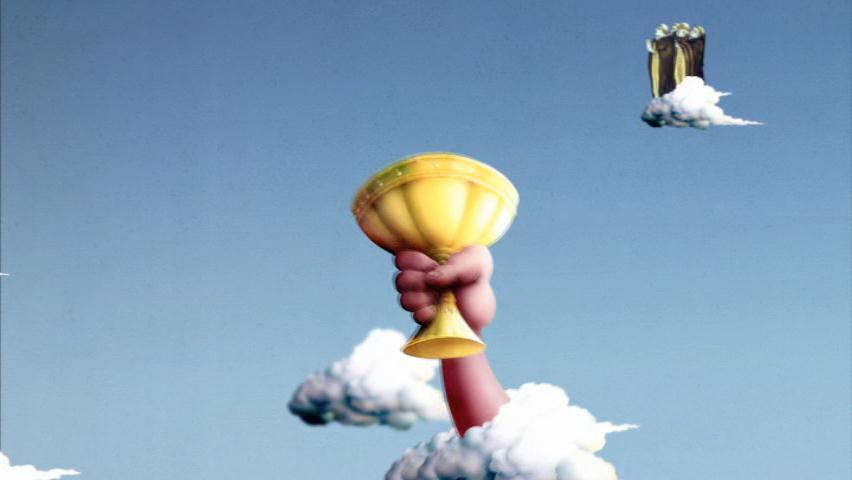
\includegraphics[width=0.8\textwidth]{grail.jpg}
  %\caption[Voorbeeld figuur.]{\label{fig:grail}Voorbeeld van invoegen van een figuur. Zorg altijd voor een uitgebreid bijschrift dat de figuur volledig beschrijft zonder in de tekst te moeten gaan zoeken. Vergeet ook je bronvermelding niet!}
%\end{figure}

%\begin{listing}
  %\begin{minted}{python}
    %import pandas as pd
   % import seaborn as sns

   % penguins = sns.load_dataset('penguins')
    %sns.relplot(data=penguins, x="flipper_length_mm", y="bill_length_mm", hue="species")
  %\end{minted}
  %\caption[Voorbeeld codefragment]{Voorbeeld van het invoegen van een codefragment.}
%\end{listing}

%\lipsum[7-20]

%\begin{table}
  %\centering
  %\begin{tabular}{lcr}
   % \toprule
    %\textbf{Kolom 1} & \textbf{Kolom 2} & \textbf{Kolom 3} \\
   % $\alpha$         & $\beta$          & $\gamma$         \\
   % \midrule
    %A                & 10.230           & a                \\
    %B                & 45.678           & b                \\
    %C                & 99.987           & c                \\
   % \bottomrule
  %\end{tabular}
  %\caption[Voorbeeld tabel]{\label{tab:example}Voorbeeld van een tabel.}
%\end{table}

Dit hoofdstuk vervolgt de probleemstelling uit de inleiding en richt zich op de wetenschappelijke en technologische vooruitgangen met betrekking tot voorspellend onderhoud en machine learning. In de inleiding werd het probleem van kleine bouwbedrijven toegelicht, maar hier wordt de huidige onderzoeksstatus binnen het bredere domein van data-gedreven onderhoudssystemen onderzocht. Deze literatuurstudie biedt de theoretische en methodologische fundamenten voor de benadering die in het volgende hoofdstuk wordt toegelicht.

\newpage

\section{\IfLanguageName{dutch}{Onderhoudsstrategieën}{Maintenance strategies}}%
\label{sec:Onderhoudsstrategieën}

Onderhoudsstrategieën worden meestal ingedeeld in reactief, preventief en predictief onderhoud. Bij reactief onderhoud wordt er pas actie ondernomen nadat er een storing is ontstaan, terwijl preventief onderhoud plaatsvindt volgens vooraf bepaalde intervallen, ongeacht de werkelijke conditie van de machine \autocite{Mikulic2024, Morganti2024}. Het onderzoek van \textcite{Deepak2025} benadrukt dat beide strategieën aanzienlijke beperkingen hebben. Reactief onderhoud kan resulteren in plotselinge stilstand, een vermindering van de productie en aanzienlijke kosten voor reparaties, terwijl preventief onderhoud kan leiden tot onnodige vervanging van nog goed werkende componenten.

%Onderhoudsstrategieën worden doorgaans ingedeeld in reactief, preventief en predictief onderhoud. Reactief onderhoud betekent dat er actie wordt ondernomen nadat een defect is ontstaan, terwijl preventief onderhoud gebeurt op vooraf bepaalde tijden, ongeacht de werkelijke conditie van de machine \autocite{Mikulic2024, Morganti2024}. Volgens het onderzoek van \textcite{Deepak2025} hebben de twee strategieën hun nadelen, namelijk reactief onderhoud kan leiden tot onvoorziene stilstand en aanzienlijke kosten, terwijl preventief onderhoud kan leiden tot onnodige vervanging van onderdelen.

Voorspellend onderhoud biedt een optie waarbij beslissingen over onderhoud worden genomen op basis van de huidige staat van een machine. Voor dit doel wordt sensordata verzameld en geanalyseerd, zodat defecten vroegtijdig kunnen worden opgemerkt en onderhoud alleen plaatsvindt wanneer dit echt nodig is \autocite{Carvalho2019}. Volgens onderzoek resulteert deze onderhoudsstrategie in een grotere beschikbaarheid van de bouwmachines, dalende onderhoudskosten en een betere planning van onderhoud van de machines \autocite{ErRatby2025, Mahale2025}. Het onderzoek van \textcite{Mahfoud2025} toont bovendien aan dat het verminderen van ongeplande stilstanden een cruciale rol speelt in de operationele resultaten van ondernemingen.

%Predictieve onderhoud richt zijn beslissingen over onderhoud op de huidige toestand van de apparatuur, die wordt gemeten met sensoren en geanalyseerd met behulp van data-analysemethoden \autocite{Carvalho2019}. De studie van \textcite{ErRatby2025} stelt dat predictieve onderhoud de toegankelijkheid van machines aanzienlijk kan verbeteren en de onderhoudskosten kan verlagen. Het onderzoek van \textcite{Mahale2025} toont aan dat predictieve onderhoud in industriële omgevingen resulteert in efficiëntere planning, een hogere betrouwbaarheid en lagere kosten.

Hoewel voorspellend onderhoud al met succes in diverse industriële sectoren wordt ingezet, is de uitvoering ervan in de bouwsector nog steeds beperkt \autocite{Mikulic2024}. Vooral kleine bouwbedrijven hebben vaak minder digitale infrastructuur en slaan minder historische sensordata op, wat het lastig maakt om geavanceerde onderhoudssystemen toe te passen. Dit leidt tot de behoefte om  machine learning-technieken te analyseren die ook nuttig zijn in contexten waarin er slechts een beperkte hoeveelheid gelabelde gegevens beschikbaar is.

%In de bouwsector is de toepassing van geavanceerde onderhoudssystemen echter minder vergevorderd dan in productieomgevingen \autocite{Mikulic2024}. Wat een kans biedt voor onderzoek binnen de sector van kleine bouwbedrijven.

\newpage

\section{\IfLanguageName{dutch}{Machine learning binnen voorspellend onderhoud}{Machine learning in predictive maintenance}}%
\label{sec:{Machine learning binnen voorspellend onderhoud}
    
Machine learning is essentieel voor hedendaagse voorspellend onderhoudssystemen. In plaats van alleen vaste onderhoudsintervallen toe te passen, worden algoritmen ingezet om patronen in sensordata te herkennen, anomalieën te waarnemen en mogelijke defecten op tijd te herkennen. Volgens het onderzoek van \textcite{Carvalho2019} zijn supervised learning, unsupervised learning en deep learning de meest gebruikte methoden voor voorspellend onderhoud. Deze methoden worden toegepast voor onder andere het opsporen van fouten, het identificeren van afwijkingen en het voorspellen van de Remaining Useful Life of RUL van machineonderdelen.

Bij supervised learning worden modellen getraind met gelabelde data, waarbij voor elke observatie duidelijker wordt of er een storing of defect is. Dit stelt modellen in staat om toekomstige defecten of storingen te categoriseren of zelfs te voorspellen. De studies van \textcite{Carvalho2019} en \textcite{Elahi2023} stellen dat, hoewel deze methode vaak uitstekende resultaten oplevert, zij sterk afhankelijk is van de aanwezigheid van voldoende gelabelde historische fouten, die in de praktijk vaak moeilijk toegankelijk zijn.

Unsupervised learning biedt een oplossing wanneer dergelijke gelabelde fouten niet aanwezig zijn. Deze modellen leren alleen het gebruikelijke gedrag van een machine en zien waarnemingen die aanvankelijk van deze norm afwijken als mogelijke afwijkingen. Volgens de onderzoeken van \textcite{Giannoulidis2024} en \textcite{Elahi2023} is deze methode zeer geschikt voor industriële toepassingen waarin er slechts een beperkte of geen gelabelde storingsdata beschikbaar zijn.

Bovendien worden deep learning-technieken steeds belangrijker in voorspellend onderhoud. De studies van \textcite{Li2025} en \textcite{Aggarwal2025} laten zien dat neurale netwerken in staat zijn om ingewikkelde patronen en tijdelijke relaties in multivariate sensorgegevens te ontdekken, wat hen geschikt maakt voor het analyseren van tijdsreeksen die afkomstig zijn van industriële machines.

Omdat er tijdens dit onderzoek slechts een beperkte hoeveelheid gelabelde sensordata beschikbaar was, ligt de focus op technieken voor het opsporen van anomalieën. Daarom worden zowel supervised model als diverse unsupervised machine learningmodellen bestudeerd en met elkaar vergeleken.

%Machine learning is van groot belang in hedendaagse predictieve onderhoudssystemen. Het onderzoek van \textcite{Carvalho2019} stelt dat supervised learning, unsupervised learning en deep learning als de voornaamste methoden voor het detecteren van fouten en het voorspellen van Remaining Useful Life of RUL van een onderdeel.

\newpage

\section{\IfLanguageName{dutch}{Supervised learning}{supervised learning}}%
\label{sec:{supervised learning}

Bij supervised learning worden machine learning-modellen getraind met gelabelde data, waarbij elke observatie aangeeft of er een defect of storing is. Dit leert de modellen hoe sensordata samenhangen met bijbehorende foutlabels, zodat ze nieuwe observaties kunnen indelen of toekomstige defecten kunnen voorspellen. Volgens het onderzoek van \textcite{Carvalho2019} is onder andere Support Vector Machines, Random Forests en Artificial Neural Networks de meest toegepaste supervised learning-methoden in voorspellend onderhoud.

Random Forest is een ensemble-algoritme dat uit verschillende beslissingsbomen bestaat en bekendstaat om zijn robuustheid, uitstekende classificatieresultaten en sterke weerstand tegen overfitting. De studies van \textcite{Carvalho2019} en \textcite{Daoudi2025} tonen aan dat dit model vaak gebruikt wordt voor het detecteren van fouten en het voorspellen van onderhoud in industriële omgevingen. 

Een belangrijk nadeel van supervised learning is echter de afhankelijkeid van gelabelde historische data. Het is belangrijk om duidelijk te maken dat dit soort datasets in industriële toepassingen vaak lastig te verkrijgen zijn, omdat storingen en defecten relatief ongebruikelijk zijn en foutlabels niet altijd op een systematische manier worden vastgelegd \autocite{Elahi2023}. Dit leidt tot een afname van de relevantie van supervised modellen in situaties waarin er slechts een beperkte hoeveelheid gelabelde sensorgegevens beschikbaar zijn.

In dit onderzoek wordt Random Forest ingezet als een gecontroleerd referentiemodel voor de openbare MetroPT-3-dataset, waarin foutlabels aanwezig zijn. De resultaten van dit model daarna vergeleken met diverse unsupervised technieken, die ook toepasbaar zijn als er geen gelabelde defectdata aanwezig zijn.

%Supervised learning modellen zoals Support Vector Machines, Random Forests en Artificial Neural Networks worden vaak gebruikt wanneer er gelabelde foutdata beschikbaar zijn \autocite{Carvalho2019}. Volgens het onderzoek van \textcite{Elahi2023} hebben echter deze modellen behoefte aan voldoende representatieve foutvoorbeelden, wat in veel realistische situaties een probleem vormt. De studie van \textcite{Roehrich2024} laat zien dat supervised learning-modellen uitstekend presteren in gecontroleerde industriële omgevingen, maar kwetsbaar zijn voor veranderingen in de dataset en een beperkte toepasbaarheid.

\newpage

\section{\IfLanguageName{dutch}{Unsupervised learning en anomaly detection}{Unsupervised learning and anomaly detection}}%
\label{sec:{unsupervised learning}
    
Als gelabelde fouten beperkt of helemaal ontbreken, kunnen unsupervised learning-methoden een geschikt alternatief bieden voor supervised learning. In tegenstelling tot supervised modellen leren deze algoritmen alleen de eigenschappen van normaal machinegedrag, zonder gebruik te maken vanop voorhand gelabele defecten. De onderzoeken van \textcite{Carvalho2019} en \textcite{Giannoulidis2024} stellen dat afwijkingen van dit gebruikelijke gedrag daarna worden gezien als mogelijke anomalieën die kunnen duiden op een eerste storing of defect.

Deze aanpak is zeer geschikt voor industriële toepassingen waar storingen relatief ongebruikelijk zijn en historische foutlabels slechts in beperkte mate beschikbaar zijn \autocite{Elahi2023}. Daarnaast toont het onderzoek van \textcite{Giannoulidis2024} aan dat het opsporen van onzichtbare afwijkingen een effectieve methode is voor voorspellend onderhoud, vooral wanneer alleen sensordata van gebruikelijke bedrijfsomstandigheden beschikbaar zijn.

Recent onderzoek toont daarnaast aan dat diverse unsupervised en deep learning-methoden met succes worden ingezet voor het opsporen van anomalieën in tijdsreeksen. Voorbeelden hiervan zijn Isolation Forest, Autoencoders, LSTM Autoencoders en One-Class Support Vector Machines, die elk op een andere wijze het gebruikelijke gedrag van machines modelleren en afwijkingen opsporen \autocite{Carvalho2019, Elahi2023, Giannoulidis2024}. Deze methoden zijn de fundamenten van de machine learning-methodiek die in dit onderzoek wordt beoordeeld.
    
%In gevallen waarin foutlabels schaars of niet volledig zijn, worden unsupervised learning-technieken gebruikt. Deze modellen leren het gebruikelijke gedrag van een machine en herkennen afwijkingen als anomalieën \autocite{Giannoulidis2024}. Autoencoders worden vaak gebruikt om verborgen weergaven van normaal gedrag te simuleren. Het onderzoek van \textcite{Aggarwal2025} presenteert DASTAD, een self-supervised transform\-er-gebaseerde aanpak voor het opsporen van onregelmatigheden in multivariate tijdsreeksen. Hun bevindingen laten zien dat transf\-ormer-architecturen effectiever complexe tijdsgebonden afhankelijkheden kunnen modelleren ten opzichte van traditionele recurrente netwerken. In de studie van \textcite{Holtz2025} combineren ze unsupervised anomaly detection met active learni\-ng, waardoor menselijke betrokkenheid alleen nodig is in gevallen van twijfel. Dit vermindert de nood aan uitgebreide labeling aanzienlijk.

\newpage

\section{\IfLanguageName{dutch}{Random Forest-model}{Random Forest-model}}%
\label{sec:{Random Forest-model}
    
Random Forest is een supervised machine learning-algoritme dat bestaat uit een set beslissingsbomen. Bij het trainen bestaat elke beslissingsboom uit een willekeurige steekproef van de trainingsdata en een willekeurige keuze van kenmerken. Volgens het onderzoek van \textcite{Carvalho2019} is de uiteindelijke voorspelling afhankelijk van de gezamenlijke keuze van alle bomen, wat resulteert in een robuuster model dan een individuele beslissingsboom en minder kwetsbaar is voor overfitting.

In voorspellend onderhoud wordt Random Forest vaak gebruikt om de condities van de machine te classificeren en defecten voor te stellen op basis van sensordata. Het onderzoek van \textcite{Carvalho2019} stelt dat Random Forest één van de meest populaire machine learning-algoritmen voor voorspellend onderhoud, dankzij de minimale behoefte aan parameterafstemming en de capaciteit om zowel lineaire als niet-lineaire relaties in de data te simuleren.

Recente onderzoeken ondersteunen deze conclusies. Random forest levert betrouwbare resultaten op bij het voorspellen van storingen in industriële compressoren en presteert het beter dan andere traditionele machine learning-modellen \autocite{Daoudi2025}. Volgens de studie van \textcite{Roehrich2024} is Random Forest zeer geschikt voor toepassingen waarbij meerdere sensoren tegelijkertijd worden ingezet, omdat het model in staat is om een grote hoeveelheid multivariate sensordata effectief te verwerken.

Een belangrijk nadeel van Random Forest is dat het een supervised leermodel is, wat betekent dat het afhankelijk is van voldoende gelabelde trainingsdata waarin gebruikelijke situaties en fouten correct zijn weergegeven. Het onderzoek van \textcite{Elahi2023} stelt dat het vaak een aanzienlijke uitdaging om dergelijke foutlabels in industriële toepassingen te vinden, vooral binnen kleine bedrijven waar historische onderhoudsdata doorgaans moeilijk toegankelijk is.

Hoewel er een nadeel is, wordt Random Forest in dit onderzoek gebruikt als referentiemodel. Het model fungeert als een populaire benchmark in de literatuur en maakt het mogelijk om de resultaten van supervised learning te vergelijken met diverse unsupervised anomaliedetectie-modellen, die beter geschikt zijn voor situaties waarin er slechts een kleine hoeveelheid of geen gelabelde defectdata beschikbaar is.
    
%Door de groei van sensorgegevens krijgen deep learning-modellen steeds meer waarde binnen predictieve onderhoud. Het onderzoek van \textcite{Li2025} laat zien dat transformer-gebaseerde modellen bijzonder geschikt zijn voor het onderzoeken van multivariate tijdsreeksen. In tegenstelling tot conventionele LSTM-netwerk\-en zijn transformers in staat om lange afstandsafhankelijkheden efficiënter te simuleren. Het onderzoek van \textcite{Mahfoud2025} benadrukt dat deep learning vooral voordelen oplevert in ingewikkelde systemen met een hoge dimensie en niet-lineaire interacties tussen variabelen. De studie van \textcite{Elahi2023} wijst echter op de hoge computationele vereisten van deep learning-modellen, wat van belang is in situaties met een beperkte IT-infrastructuur.

\newpage

\section{\IfLanguageName{dutch}{Isolation Forest-model}{Isolation Forest-model}}%
\label{sec:{Isolation Forest-model}

Isolation Forest is een unsupervised machine learning-algoritme dat speciaal is ontworpen voor het opsporen van afwijkingen. In tegenstelling tot supervised modellen heeft Isolation Forest tijdens de training geen gelabelde fouten nodig. Het algoritme veronderstelt dat afwijkende observaties eenvoudiger kunnen worden geïsoleerd dan gerbuikelijke observaties. Volgens het onderzoek van \textcite{Carvalho2019} moet er voor dit doel willekeurige beslissingsbomen gevormd worden, waaarbij afwijkingen meestal met minder splitsingen worden gerealiseerd dan gebruikelijke datapunten.

Binnen voorspellend onderhoud wordt Isolation Forest steed meer gebruikt om afwijkingen in sensorgegevens te identificeren wanneer historische foutlabels beperkt of niet toegankelijk zijn. Volgens het onderzoek van \textcite{Carvalho2019} is Isolation Forest één van de meest populaire methoden voor het opsporen van onzichtbare afwijkingen, door de eenvoudige uitvoering, de korte rekentijd en de capaciteit om grote hoeveelheden sensordata effectief te bestuderen.

Unsupervised methoden, zoals Isolation Forest, zijn bijzonder geschikt voor industriële toepassingen waarin defecten slechts af en toe voorkomen en gelabelde foutgegevens beperkt zijn \autocite{Elahi2023}. Volgens de studie van \textcite{Giannoulidis2024} is het ook mogelijk om anomalieën te detecteren op basis van normaal machinegedrag, wat een waardevolle oplossing biedt voor voorspellend onderhoud wanneer alleen sensordata van de gebruikelijke machinecondities beschikbaar zijn.

Een voordeel van Isolation Forest is dat het zonder voorafgaande kennis van storingen of defecten in staat is om afwijkende patronen te herkennen. Het model is bovendien realtief snel te trainen en kan goed worden geschaald naar grotere datasets. Een nadeel is dat het algoritme afwijkingen opmerkt op basis van statische isolatie, wat betekent dat niet elke waargenomen afwijking noodzakelijk gelijkstaat aan een daadwerkelijk defect. Volgens de onderzoeken van \textcite{Carvalho2019} en \textcite{Elahi2023} zijn de prestaties daarnaast afhankelijk van de gekozen modelparameters en de kwaliteit van de beschikbare sensordata.

In dit onderzoek wordt Isolation Forest beschreven als het eerste unsupervised referentiemodel voor het opsporen van anomalieën. Het model wordt gebruikt voor zowel de openbare MetroPT-3-dataset als de private tractordataset om te onderzoeken in hoeverre afwijkingen kunnen worden vastgelegd zonder gebruik te maken van gelabelde foutdata. Dit maakt het mogelijk om de toepasbaarheid van deze techniek in kleine bouwbedrijven te evalueren.

%Een cruciale uitdaging in voorspellend onderhoud is de kwaliteit van gegevens. Ruis en signaalvervorming oefenen een aanzienlijke negatieve invloed uit op de prestaties van modellen voor foutdetectie \autocite{Wang2025}. In industriële omgevingen, vooral in de bouwsector, worden sensoren geconfronteerd met stof, trillingen en temperatuurfluctuaties \autocite{Mikulic2024}. Het onderzoek van \textcite{Nayak2024} benadrukt dat feature engineering en signaalverwerking essentiële stappen zijn voor het creëren van betrouwbare modellen, want zonder voldoende preprocessing kunnen zelfs geavanceerde modellen onjuiste voorspellingen genereren.

\newpage

\section{\IfLanguageName{dutch}{Autoencoder-model}{Autoencoder-model}}%
\label{sec:{Autoencoder-model}
    
Een Autoencoder is een unsupervised deep learning-model dat bedoeld is om de normale kenmerken van data te leren zonder gelabelde foutvoorbeelden te gebruiken. Het netwerk bestaat uit een encoder, die de invoerdata samenperst tot een compacte weergave. De decoder probeert daarna de oorspronkelijke invoer weer te herstellen. Als het model alleen getraind is op normale machinecondities, kan het deze data goed reconstrueren. Het onderzoek van \textcite{Carvalho2019} zegt wel dat bij afwijkende of defecte situaties de reconstructiefout groter wordt, waardoor afwijkingen worden gevonden.

Autoencoders worden steeds vaker ingezet voor voorspellend onderhoud, omdat industriële datasets vaak slechts een beperkt aantal gelabelde defectdata bevatten. Autoencoders bieden een effectieve manier om afwijkingen te detecteren, omdat het model het gebruikelijke gedrag van een machine leert en daarna afwijkingen kan opsporen zonder dat er vooraf kennis is van bepaalde defecten \autocite{Giannoulidis2024}. Dit maakt ze bijzonder geschikt voor industriële toepassingen waar storingen zelden voorkomen of niet goed zijn vastgelegd.

Autoencoders kunnen met succes worden gebruikt voor het voorspellen van onderhoud op tijdsreeksdata. Dit wordt ook bevestigt in de studie van \textcite{Davari2021} naar de MetroPT-3-dataset waarin een methode voor anomaliedetectie ontwikkeld die gebruikmaakt van deep learning om afwijkingen in sensordata van een luchtcompressorsysteem op tijd te herkennen. Daaruit bleek dat autoencoders een nuttig alternatief zijn voor conventionele supervised classificatiemodellen, vooral wanneer foutlabels slechts in beperkte mate beschikbaar zijn.

Een cruciaal voordeel van autoencoders is dat ze in staat zijn om ingewikkelde, niet-lineaire interacties tussen diverse sensoren te simuleren. Dit stelt hen in staat om meer nauwkeurige veranderingen in multivariate sensorgegevens te herkennen dan veel traditionele machine learning-algoritmen \autocite{Carvalho2019}. Bovendien is het niet noodzakelijk om defecten grondig te labelen, wat de toepasbaarheid binnen kleine bouwbedrijven vergroot. Volgens het onderzoek van \textcite{Giannoulidis2024} is een nadeel dat de prestaties aanzienlijk afhankelijk zijn van de gekozen netwerkarchitectuur, de trainingsparameters en het vaststellen van een passende reconstructiedrempel om normale en afwijkende situaties van elkaar te onderscheiden.

In dit onderzoek wordt de Autoencoder gebruikt als één van de voornaamste anomaliedetectiemodellen. Het model wordt eerst beoordeeld op basis van de openbare MetroPT-3-dataset en daarna geïmplementeerd op een privédataset van een tractor die in grondverzet- en transportsector wordt ingezet. Zo wordt nagegaan in hoeverre een Autoencoder geschikt is om anomalieën in sensordata te herkennen, zodat het onderhoudsbeleid van bouwmachines in kleine bouwbedrijven kan worden ondersteund.
    
%Een terugkerend probleem voor kleine bedrijven is het gebrek aan uitgebreide historische datasets. Kleine datavolumes worden beschouwd als één van de belangrijkste obstakels voor de implementatie van AI \autocite{Elahi2023}. Het onderzoek van \textcite{Meddaoui2024} bewijst dat Generatieve Adversarial Networks of GANs kunnen worden gebruikt om synthetische sensorgegevens te creëren voor het trainen van predictieve onderhoudsmodellen. Dit concept wordt ook verbonden met digital twins, waarbij gesimuleerde omgevingen worden ingezet voor het modelleren van falingsscenario's \autocite{Hu2024}. Volgens de studie van \textcite{Nieminen2026} worden synthetische gegevens steeds vaker gebruikt om modellen te evalueren wanneer er beperkte beschikbaarheid is aan reële foutdata.

\section{\IfLanguageName{dutch}{LSTM Autoencoder-model}{LSTM Autoencoder-model}}%
\label{sec:{LSTM Autoencoder-model}
    
Een LSTM Autoencoder is een variant van de traditionele autoencoder die gebruiktmaakt van Long Short-Term Memory-netwerken of LSTM. LSTM is een soort recurrent neuraal netwerk dat specifiek is ontworpen om afhankelijkheden in verschillende tijdsperiodes te identificeren. Het onderzoek van \textcite{Carvalho2019} stelt het model in staat om niet alleen de verbanden tussen diverse sensoren te begrijpen, maar ook de ontwikkeling van sensormetingen in de loop der jaren te analyseren.

In het kader van voorspellend onderhoud worden sensordata meestal in opeenvolgende tijdsperiodes verzameld, waarbij veranderingen zich langzaam voordoen. Deep learning-modellen die tijdelijke afhankelijkheden in overweging nemen, zijn effectiever voor het bestuderen van ingewikkelde multivariate sensorgegevens dan trditionele machine learning-modellen \autocite{Li2025}. LSTM-netwerken zijn in staat om zowel kortetermijn- als langetermijnpatronen te identificeren, wat het mogelijk maakt om kleine afwijkingen die wijzen op een defect sneller te ontdekken.

De integratie van een LSTM-netwerk met een Autoencoder maakt het mogelijk om het gebruikelijke van een machine, dat afhankelijk is van tijd, opnieuw te creëren. Tijdens de training leert het model alleen gebruik te maken van normale sequenties van sensordata. Als er tijdens de inferentie een afwijkende sequentie wordt gepresenteerd, neemt de reconstructiefout toe, wat kan leiden tot het vaststellen van een mogelijke anomalie. Volgens de studie van \textcite{Davari2021} biedt deze methode een effectieve manier om anomalieën te identificeren in industriële tijdsreeksen waarvoor slechts een beperkte hoeveelheid gelabelde fouten beschikbaar is.

Een cruciaal voordeel van een LSTM Autoencoder is dat het model in staat is om zowel de ruimtelijke relaties tussen sensoren als de tijdelijke afhankelijkheden tussen achtereenvolgende metingen te leren. Dit maakt het mogelijk om geleidelijk ontwikkelende defecten te identificeren in vergelijking met een traditionele Autoencoder. Aan de andere kant vergen volgens de studies van \textcite{Elahi2023} en \textcite{Li2025} LSTM Autoencoders meer rekenkracht, hebben ze langere trainingstijden en zijn ze gevoeliger voor de keuze van hyperparameters, zoals de lengte van de sequentie, het aantal LSTM-eenheden en het aantal iteraties bij de training.

In dit onderzoek wordt de LSTM Autoencoder gebruikt als een geavanceerd model voor het detecteren van onregelmatigheden zonder supervisie. Het model wordt eerst beoordeeld op basis van de openbare MetroPT-3-dataset en daarna geïmplementeerd op de private tractordataset. Zo kan worden nagegaan of het modelleren van tijdelijke afhankelijkheden resulteert in een verbeterde detectie van afwijkingen in sensordata, wat een waardevolle aanvulling biedt voor het bevorderen van het onderhoudsbeleid van bouwmachines in kleine bouwbedrijven.
    
%Een andere ontwikkeling in voorspellend onderhoud is de overgang naar Edge AI. In plaats van alleen data in de cloud te verwerken, worden modellen op locatie op industriële apparatuur geïnstalleerd \autocite{Mahale2025}. Dit vermindert de latency en verbetert de privacy van de data.
%Het onderzoek van \textcite{Elahi2023} wijst uit dat voor kleine bedrijven een eenvoudige en effectieve modelarchitectuur van groter belang kan zijn dan optimale precisie, vanwege de beperkte infrastructuur.

\section{\IfLanguageName{dutch}{Synthese en onderzoekspositie}{Synthesis and research position}}%
\label{sec:{Synthese en onderzoekspositie}
    
Uit de literatuur blijkt dat:
\begin{itemize}
    \item Voorspellend onderhoud aantoonbare voordelen biedt ten opzichte van traditionele onderhoudsstrategieën \autocite{ErRatby2025, Mahale2025}.
    
    \item Machine learning, in het bijzonder anomaly detection, geschikt is voor foutdetectie in industriële systemen \autocite{Carvalho2019, Giannoulidis2024}.
    
    \item Deep learning en transformer-modellen sterke prestaties leveren bij complexe tijdsreeksen \autocite{Li2025, Aggarwal2025}.
    
    \item Beperkte data en ruis belangrijke implementatie-uitdagingen vormen \autocite{Elahi2023, Wang2025}.
    
    \item Synthetische data en digital twins mogelijke oplossingen bieden voor datatekorten \autocite{Meddaoui2024, Hu2024}.
\end{itemize}

Wat minder is bestudeeerd, is de specifieke toepasbaarheid van deze technieken in kleine bouwbedrijven met beperkte financiële middelen en specifieke operationele omstandigheden.

Deze bachelorproef richt zich op dit kruispunt, namelijk het samenbrengen van technieken voor anomaly detection met een praktisch toepasbaar implementatiekader voor een kleine bouwbedrijf.
%%=============================================================================
%% Methodologie
%%=============================================================================

\chapter{\IfLanguageName{dutch}{Methodologie}{Methodology}}%
\label{ch:methodologie}

%% TODO: In dit hoofstuk geef je een korte toelichting over hoe je te werk bent
%% gegaan. Verdeel je onderzoek in grote fasen, en licht in elke fase toe wat
%% de doelstelling was, welke deliverables daar uit gekomen zijn, en welke
%% onderzoeksmethoden je daarbij toegepast hebt. Verantwoord waarom je
%% op deze manier te werk gegaan bent.
%% 
%% Voorbeelden van zulke fasen zijn: literatuurstudie, opstellen van een
%% requirements-analyse, opstellen long-list (bij vergelijkende studie),
%% selectie van geschikte tools (bij vergelijkende studie, "short-list"),
%% opzetten testopstelling/PoC, uitvoeren testen en verzamelen
%% van resultaten, analyse van resultaten, ...
%%
%% !!!!! LET OP !!!!!
%%
%% Het is uitdrukkelijk NIET de bedoeling dat je het grootste deel van de corpus
%% van je bachelorproef in dit hoofstuk verwerkt! Dit hoofdstuk is eerder een
%% kort overzicht van je plan van aanpak.
%%
%% Maak voor elke fase (behalve het literatuuronderzoek) een NIEUW HOOFDSTUK aan
%% en geef het een gepaste titel.

Dit onderzoek hanteert een praktische en casusgerichte benadering om zowel probleemgerichte als oplossingsgerichte vragen te beantwoorden.
De aanpak past bij de bestaande technieken voor voorspellend onderhoud, zoals gebruikt in eerdere case-en vergelijkende studies van anderen. Deze bachelorproef zal ongeveer veertien weken in beslag nemen. Enkele weken zullen elkaar overlappen, dit wordt hieronder verder uitgelegd in de verschillende fases.

\section{\IfLanguageName{dutch}{Literatuurstudie}{literature study}}%
\label{sec:literatuurstudie_methodologie}

In de eerste plaats wordt er een literatuurstudie uitgevoerd om het onderhoudsprobleem in de bouwsector beter te kunnen plaatsen en te
onderzoeken waarom gangbare onderhoudsmethoden leiden tot stilstand en fouten. Dit is al bewezen in de industrie en bij bouwmachines \autocite{ErRatby2025, Farwaha2024, Mikulic2024}. Bovendien wordt onderzocht welke sensoren, datatypes en machine learning- en unsupervised learning-algoritmes momenteel het meest effectief zijn voor het opsporen van fouten en het voorspellen van de resterende levensduur van bepaalde machinecomponenten \autocite{Carvalho2019, Li2025, Meddaoui2024, Nayak2024}. Deze fase zal ongeveer drie weken duren en een mogelijke overlap met andere fases kan ontstaan als er
extra bronnen vereist zijn. Daarnaast kan er een deliverable worden opgesteld dat aan het einde van deze drie weken ingediend kan worden om een heldere deadline te stellen.

\section{\IfLanguageName{dutch}{Analyse-fase}{analysis phase}}%
\label{sec:analyse-fase}

In deze fase wordt de specifieke situatie bij Bouwonderneming Marchand BV onderzocht, in samenwerking met het bedrijf, door
middel van gesprekken met de technische verantwoordelijke.
Deze methode is gebaseerd op de praktijkvoorbeelden uit de onderhoudsonderzoeken van \textcite{Racchumi2024} en \textcite{Deepak2025}. De meest voorkomende problemen, onderhoudsintervallen en de belangrijkste sensoren worden hierbij bepaald. Het uitwerken van deze fase zal naar verwachting één tot twee weken in beslag nemen, met mogelijke overlap met de literatuurstudie.
    
\section{\IfLanguageName{dutch}{Data verzameling en data captatie }{Data collection and data recording}}%
\label{sec:data-verzameling-en-data-captatie}

Onderhouds- en foutgegevens kunnen opgevraagd worden bij de machinedealers, omdat kleine bouwbedrijven vaak geen
eigen sensorgegevens registreren. In de studies
van \textcite{Elahi2023}, \textcite{Hu2024} en \textcite{Wang2025} over voorspellend onderhoud is het gebruikelijk om informatie te verkrijgen van externe organisaties waaronder dealers van de machines. Als dat nodig is, kunnen er extra gesimuleerde of synthetische tijdreeksen of data worden gecreëerd op basis van eerder bekende faalpatronen uit de literatuur\autocite{Meddaoui2024, Nayak2024, Wang2025}. Er bestaat een kans dat sommige dealers geen toegang willen geven tot hun data, daarom is er een alternatieve aanpak uitgewerkt in een volgende sectie van de methodologie namelijk de sectie ‘Risico en alternatieve aanpak‘ gebaseerd op synthetische data. Voor het opstellen van een complete dataset wordt ongeveer vier weken besteed, inclusief het bezoeken en contacteren van de diverse dealers en indien nodig het simuleren van extra bijkomende data. Ondertussen werd er voor de start van de bachelorproefperiode al contact gelegd met de verantwoordelijke van Bouwonderneming Marchand BV en werd ook al contact gelegd naar een aantal dealers van bouwmachines zoals onder andere Van Der Spek in Ternat, een dealer van één van de hijskranen in het bedrijf.

\section{\IfLanguageName{dutch}{Preprocessing en feature engineering }{Preprocessing and feature engineering}}%
\label{sec:preprocessing-and-feature-engineering}

In deze fase worden de verzamelde gegevens weergegeven, gefilterd en klaargemaakt voor gebruik in een unsupervised learning-model. Dit omvat onder andere het verwijderen van eventuele ruis uit de dataset en het normaliseren van tijdsreeksen, methoden die volgens de onderzoeken van \textcite{Wang2025} en \textcite{Aggarwal2025} essentieel worden beschouwd voor foutdiagnose onder realistische situaties. \textcite{Nayak2024} en \textcite{Dang2024} stellen dat de feature engineering gebaseerd is op de best practices voor gegevens die afkomstig zijn van vibratiesensoren, belastingsensoren en multisensoren. Voor deze fase is er ongeveer een week nodig om de dataset klaar te maken voor de volgende fase.

\section{\IfLanguageName{dutch}{Proof-of-concept machine learning-model}{Proof-of-concept machine learning-model(ENG)}}%
\label{sec:proof-of-concept machine learning-model}

Er worden diverse machine learning-algoritmes ontwikkeld en beoordeeld om onderhoudsbehoeften te voorspellen op basis van sensorgegevens. Volgens \textcite{Elahi2023}, \textcite{Giannoulidis2024} en \textcite{Aggarwal2025} is gelabelde foutdata bij kleine bouwbedrijven vaak beperkt en richt
men zich voornamelijk op unsupervised en selfsupervised technieken, die het mogelijk maken om afwijkingen in sensorgegevens te identificeren zonder duidelijke labels. De bestudeerde algoritmen omvatten similarity-based methoden zoals Cosinus‐similariteit, forecasting-based modellen voor tijdsreeksen zoals LSTM, deep unsupervised modellen zoals autoencoders en een self-supervised Transformer (DASTAD) voor anomaly detection in multivariate
sensordata \autocite{Aggarwal2025, Giannoulidis2024}. Volgens \textcite{Carvalho2019}, \textcite{Li2025} en \textcite{Khalili2025} bieden verschillende supervised learning modellen, zoals Random Forests, Gradient Boosting en CatBoost ook goede resultaten bij voldoende gelabelde gegevens. Stel dat de sensordata voldoende labeling bevat, kunnen de resultaten van de supervised learning modellen ook bestudeerd en beoordeeld worden. De uitvoering vindt plaats in Python met Pandas, Scikit-learn en PyTorch en er wordt gekeken in welke mate tijdreeksmodellen uit andere domeinen,
zoals multiview time-seriesmodellen voor voertuigen, relevant zijn voor bouwmachines \autocite{Chen2025}. Voor deze fase zijn er ongeveer twee weken gepland.

\section{\IfLanguageName{dutch}{Beoordeling van het model}{assessment of the model}}%
\label{sec:beoordeling-van-het-model}

In deze fase wordt het model geëvalueerd met gebruikelijke prestatie-indicatoren zoals precision, recall, F1-score en confusion-matrices zoals aanbevolen in de studies over foutclassificatie en onderhoudsdetectie \autocite{Mahale2025, Roehrich2024}. De resultaten worden vergeleken met het bestaande preventieve onderhoudsbeleid van het bouwbedrijf. Volgens \textcite{Deepak2025} en \textcite{Hu2024} richt men zich op onjuiste meldingen, overbodige waarschuwingen en de relevantie van de resultaten in een realistische situatie voor het bouwbedrijf. Voor deze fase wordt ongeveer een week beschikbaar gesteld om een grondige evaluatie van het model te maken.

\section{\IfLanguageName{dutch}{Risico en alternatieve aanpak}{Risk and alternative approach}}%
\label{sec:risico-en-alternatieve-aanpak}

Bij het uitvoeren van deze bachelorproef wordt in overweging genomen dat historische sensorgegevens van machine-dealers mogelijk niet toegankelijk zijn of ze deze data niet willen vrijgeven. In zulke gevallen wordt volgens \textcite{Carvalho2019} en \textcite{Elahi2023} in de literatuur vaak gebruikgemaakt van synthetische of gesimuleerde data als een haalbaar en wetenschappelijk onderbouwd alternatief, vooral in het voorspellend onderhoud in industriële omgevingen. Synthetische gegevens maken het mogelijk om realistische sensorgegevens te creëren, gebaseerd op bekende gedragingen van de machines, slijtagepatronen en faalmechanismen. Bij diverse onderzoeken van \textcite{Meddaoui2024}, \textcite{Nayak2024} en \textcite{Wang2025} wordt deze methode gebruikt om proof-of-concept modellen te creëren en algoritmische beslissingen te verifiëren, vooral wanneer real-world gegevens beperkt, onvolledig of vertrouwelijk zijn. Hoewel modellen die alleen op synthetische gegevens worden getraind niet alle complexiteit en ruis van realistische werkomgevingen bevatten, wijzen recente studies erop dat unsupervised en self-supervised leermethoden minder afhankelijk zijn van exacte labeling, wat resulteert in een betere generalisatie van gesimuleerde naar echte gegevens, vooral voor het opsporen van anomalieën \autocite{Aggarwal2025, Holtz2025}. \textcite{Hu2024} en \textcite{Maguluri2024} verklaren ook in hun onderzoeken dat digitale tweelingen en gesimuleerde omgevingen bovendien steeds vaker worden toegepast om synthetische datasets te genereren die sterk lijken op de werkelijke processen. In deze bachelorproef worden synthetische gegevens gezien als een volwaardige alternatieve aanpak om de technische haalbaarheid van een voorspellend onderhoudsmodel aan te tonen. Volgens \textcite{Raffaele2024} en \textcite{ErRatby2025} ligt de nadruk op het beoordelen van geschikte algoritmen, methoden voor dataverwerking en evaluatiestrategieën, wat in de literatuur wordt gezien als een gebruikelijke en gangbare aanpak binnen een proof-of-concept situatie. Als deze alternatieve aanpak uitgevoerd wordt omdat de machine-dealers de data niet wensen vrij te gegeven of geen toegang hebben, wordt voor deze fase hetzelfde aantal weken ingepland zoals bij de dataverzameling fase. In plaatst van de weken te gebruiken om data te verzamelen, worden deze dan gebruikt om synthetische data te creëren.

\section{\IfLanguageName{dutch}{Conclusie en implementatie voor het bouwbedrijf}{conclusion and implementation for the construction company}}%
\label{sec:Conclusie-en-implementatie-voor-het-bouwbedrijf}

In deze laatste fase worden de resultaten beoordeeld en wordt er een technisch en praktisch adviesrapport opgesteld voor Bouwonderneming Marchand BV, het bedrijf waarmee deze bachelorproef wordt uitgevoerd. De impact van het model is gebaseerd op literatuur die aantoont dat voorspellend onderhoud resulteert in lagere kosten, minder stilstand van machines en een hogere betrouwbaarheid van deze machines \autocite{ErRatby2025, Maguluri2024, Mahfoud2025}. Het adviesrapport en het proof-of-concept vormen samen het definitieve resultaat van de bachelorproef en kunnen als deliverables worden ingediend en gebruikt worden tijdens de mondelinge verdediging. Voor deze fase wordt ongeveer één week vrijgemaakt om de uitwerking te voltooien.




%%=============================================================================
%% Databeschikbaarheid
%%=============================================================================

\chapter{\IfLanguageName{dutch}{Databeschikbaarheid en uitdagingen bij het verkrijgen van datasets in de bouwsector}{Data availability and challenges in obtaining datasets in the construction industry}}%
\label{ch:databeschikbaarheid en uitdagingen bij het verkrijgen}

Een cruciale vereiste voor het creëren van een betrouwbaar voorspellend onderhoudsmodel is de beschikbaarheid van kwalitatieve, representatieve en voldoende uitgebreide datasets. Machine learning-algoritmes, met name modellen voor voorspellend onderhoud, zijn namelijk sterk afhankelijk van eerdere gegevens om patronen, afwijkingen en faalgedrag te herkennen. Zonder toegang tot dergelijke gegevens is het lastig om modellen te ontwikkelen die nauwkeurig en robuust zijn in praktische toepassingen. Volgens het onderzoek van \textcite{Elahi2023} is de beschikbaarheid van gegevens een essentiële vereiste voor een succesvolle invoering van kunstmatige intelligentie in industriële toepassingen.

In de bouwsector is het echter bijzonder moeilijk om dergelijke datasets te verkrijgen. In tegenstelling tot sterk gedigitaliseerde sectoren is de bouwsector historisch gezien minder afhankelijk van gegevens, wat leidt tot een lagere maturiteit op het gebied van verzameling en beheer van gegevens. Volgens de studie van \textcite{Mikulic2024} bevindt de sector zich nog in een relatief vroege fase van digitale transformatie, waardoor gestructureerde en historische opgebouwde datasets vaak ontbreken.

Bovendien onderstreept het onderzoek van \textcite{Wang2025} dat industriële gegevens vaak moeilijk bereikbaar zijn, zelfs als ze binnen organisaties aanwezig zijn. Data kan over diverse systemen worden verspreid, niet gestandaardiseerd zijn of door technische of organisatorische obstakels moeilijk bereikbaar zijn. Deze kwestie is volgens de studie van \textcite{Hu2024} nog duidelijker bij kleine en middelgrote bedrijven, waar vaak de benodigde infrastructuur en expertise voor databeheer ontbreken.

Daarnaast laten onderzoeken zien dat het niet vanzelfsprekend is om gegevens te delen tussen diverse partijen binnen een industriële omgeving. Volgens de onderzoeken van \textcite{Elahi2023} en \textcite{Wang2025} zijn organisatorische, commerciële en vertrouwelijkheidsgerelateerde elementen cruciaal voor het bepreken van de toegang tot gegevens. Dit leidt ertoe dat waardevolle datasets vaak niet beschikbaar zijn voor onderzoeksdoeleinden of externe toepassingen.

Deze bevindingen worden bevestigd door de ervaringen binnen dit onderzoek, waarbij het verkrijgen van datasets via externe partijen, zoals machine-dealers, gepaard ging met beperkte respons, onduidelijkheid over datatoegang en een lage bereidheid tot samenwerking. Deze praktische uitdagingen komen volgense de studies van \textcite{Elahi2023} en \textcite{Wang2025} overeen met de in de literatuur genoemde obstakels voor toegang tot de data en het delen van data in industriële omgevingen.

De mix van beperkte datacaptatie, beperkte toegankelijkheid en terughoudendheid bij het delen van gegevens maakt het verzamelen van geschikte datasets tot één van de belangrijkste obstakels in dit onderzoek. Volgens de studies van \textcite{Hu2024} en \textcite{Elahi2023} heeft dit niet alleen invloed op de fase van dataverzameling, maar ook op de verdere ontwikkeling en validatie van voorspellende modellen, zoals ook wordt vermeld in de literatuur over AI-toepassingen in onderhoudssituaties.

\newpage

\section{\IfLanguageName{dutch}{Beperkte datacaptatie en digitalisering}{Limited data collection and digitization}}%
\label{sec: Beperkte datacaptatie en digitalisering}

Binnen kleine bouwbedrijven is de digitalisering van machinegegevens vaak nog niet optimaal. In tegenstelling tot volledig geautomatiseerde industriële omgevingen, waar sensorgegevens voortdurend en op een systematische manier worden verzameld en opgeslagen, hebben veel bouwbedrijven geen uitgebreide historische datasets. Dit ontbreken van datacaptatie vormt een cruciale obstakel voor het gebruik van technieken die gebaseerd zijn op gegevens, zoals voorspellend onderhoud. Volgens het onderzoek van \textcite{Elahi2023} is het beschikbaar hebben van gestructureerde en voldoende grote datasets een essentiële vereiste voor de invoering van kunstmatige intelligentie in industriële toepassingen.

De beperkte dataverzameling in de bouwsector is nauw verbonden met de lagere graad van digitalisering binnen de sector. Het onderzoek van \textcite{Mikulic2024} stelt dat de bouwsector achterloopt ten opzichte van andere sectoren op het gebied van digitale ontwikkeling, wat onder andere blijkt uit een beperkte integratie van sensoren, IoT-technologieën en centrale dataplatformen. Volgens de onderzoeken van \textcite{Mikulic2024} en \textcite{Hu2024} leidt dit ertoe dat operationele gegevens van machines vaak niet automatisch worden vastgelegd of slechts gedeeltelijk worden bijgehouden, wat de toegankelijkheid van waardevolle gegevens vermindert.

Daarnaast wordt onderhoudsinformatie in veel gevallen nog manueel geregistreerd, bijvoorbeeld via papieren documenten of eenvoudige digitale tools zonder gestandaardiseerde structuur. Dit resulteert in onvolledige, onconsistente en lastig te verwerken datasets. De studie van \textcite{Hu2024} stelt dat het gebrek aan gestructureerde en kwalitatieve gegevens een aanzienlijke obstakel vormt voor het gebruik van machine learning-methoden, omdat deze modellen sterk afhankelijk zijn van consistente inputgegevens.

Verder onderstreept het onderzoek van \textcite{Wang2025} dat, zelfs wanneer gegevens worden verzameld, deze vaak niet op een centrale en toegankelijke wijze worden opgeslagen. Data kan over diverse systemen of afdelingen worden verspreid, waardoor het lastig is om een compleet en samenhangend overzicht te krijgen van het gedrag en de staat van machines. Volgens de studie van \textcite{Wang2025} beperkt dit probleem van gefragmenteerde datacaptatie de mogelijkheden voor geavanceerde data-analyse aanzienlijk.

De combinatie van beperkte digitalisering, onvoldoende gestructureerde data en gefragmenteerde opslag resulteert in een lage beschikbaarheid van bruikbare datasets binnen de bouwsector \autocite{Mikulic2024, Hu2024, Wang2025}. Dit vormt volgens de studies van \textcite{Elahi2023} en \textcite{Hu2024} een essentiële obstakel voor het creëren van betrouwbare voorspellende modellen, omdat zowel de hoeveelheid als de kwaliteit van de beschikbare gegevens niet genoeg zijn om complexe patronen en faalmechanismen nauwkeurig te analyseren.

\newpage

\section{\IfLanguageName{dutch}{Problemen bij het verkrijgen van externe datasets}{Problems obtaining external datasets}}%
\label{sec: problemen bij het verkrijgen van externe datasets}

Omdat kleine bouwbedrijven vaak geen uitgebreide of gestructureerde interne datasets hebben, wordt er in onderzoek en praktijk vaak gebruikgemaakt van externe bronnen van gegevens, zoals machine-dealers, fabrikanten of serviceproviders \autocite{Elahi2023, Hu2024}. In industriële omgevingen worden dergelijke gegevens vaak door diverse betrokkenen beheerd, waardoor externe partijen een mogelijke bron zijn voor operationele en onderhoudsinformatie \autocite{Meddaoui2024, Nayak2024}. In de praktijk blijkt het verwerven van deze datasets echter een ingewikkelde en onduidelijke taak te zijn.

Tijdens de uitvoering van dit onderzoek werd aangetoond dat het in contact komen met externe partijen vaak leidt tot diverse uitdagingen. In verschillende situaties was er geen reactie op contactpogingen, waardoor het opstarten van samenwerkingen lastig werd. Daarnaast werd vastgesteld dat sommige partijen expliciet geen toegang wilden geven tot hun data, terwijl in andere gevallen onduidelijk bleef of de gevraagde data überhaupt beschikbaar was. Deze beperkte respons en onduidelijkheid leiden tot een aanzienlijke vertraging en onzekerheid tijdens de fase van het verzamelen van gegevens in het onderzoek.

De literatuur toont aan dat dergelijke problemen vaak voorkomen bij het verzamelen van industriële informatie. De toegang tot gegevens wordt vaak bemoeilijkt door organisatorische en praktische obstakels, waaronder het gebrek aan standaard processen voor het delen van gegevens en een beperkte hoeveelheid interne middelen \autocite{Wang2025, Dissem2024}. Bovendien onderstreept het onderzoek van \textcite{Aggarwal2025} dat veel organisaties niet goed voorbereid zijn op het delen van gegevens voor analytische doeleinden, wat de toegankelijkheid nog verder vermindert.

Een cruciale factor hierbij is de vertrouwelijkheid van bedrijfsinformatie. Bedrijven zijn vaak niet bereid om informatie over machinegebruik, onderhoud en prestaties met externe partijen te delen, omdat deze informatie strategisch van belang is \autocite{Hu2024, Meddaoui2024}. Volgens de studies van \textcite{Elahi2023} en \textcite{Nayak2024} wordt dit versterkt door twijfels over het gebruik van gegevens, de eigendom en de mogelijke commerciële gevolgen.

%%=============================================================================
%% Databeschikbaarheid
%%=============================================================================

\chapter{\IfLanguageName{dutch}{De verkregen werkelijke data van een machine in de bouw}{Actual data collected from a machine in the construction industry}}%
\label{ch:de echte data}

test

%%=============================================================================
%% de openbare dataset
%%=============================================================================

\chapter{\IfLanguageName{dutch}{De gekozen openbare dataset}{The selected public dataset}}%
\label{ch:de openbare data}


% Voeg hier je eigen hoofdstukken toe die de ``corpus'' van je bachelorproef
% vormen. De structuur en titels hangen af van je eigen onderzoek. Je kan bv.
% elke fase in je onderzoek in een apart hoofdstuk bespreken.

%%%=============================================================================
%% Databeschikbaarheid
%%=============================================================================

\chapter{\IfLanguageName{dutch}{Databeschikbaarheid en uitdagingen bij het verkrijgen van datasets in de bouwsector}{Data availability and challenges in obtaining datasets in the construction industry}}%
\label{ch:databeschikbaarheid en uitdagingen bij het verkrijgen}

Een cruciale vereiste voor het creëren van een betrouwbaar voorspellend onderhoudsmodel is de beschikbaarheid van kwalitatieve, representatieve en voldoende uitgebreide datasets. Machine learning-algoritmes, met name modellen voor voorspellend onderhoud, zijn namelijk sterk afhankelijk van eerdere gegevens om patronen, afwijkingen en faalgedrag te herkennen. Zonder toegang tot dergelijke gegevens is het lastig om modellen te ontwikkelen die nauwkeurig en robuust zijn in praktische toepassingen. Volgens het onderzoek van \textcite{Elahi2023} is de beschikbaarheid van gegevens een essentiële vereiste voor een succesvolle invoering van kunstmatige intelligentie in industriële toepassingen.

In de bouwsector is het echter bijzonder moeilijk om dergelijke datasets te verkrijgen. In tegenstelling tot sterk gedigitaliseerde sectoren is de bouwsector historisch gezien minder afhankelijk van gegevens, wat leidt tot een lagere maturiteit op het gebied van verzameling en beheer van gegevens. Volgens de studie van \textcite{Mikulic2024} bevindt de sector zich nog in een relatief vroege fase van digitale transformatie, waardoor gestructureerde en historische opgebouwde datasets vaak ontbreken.

Bovendien onderstreept het onderzoek van \textcite{Wang2025} dat industriële gegevens vaak moeilijk bereikbaar zijn, zelfs als ze binnen organisaties aanwezig zijn. Data kan over diverse systemen worden verspreid, niet gestandaardiseerd zijn of door technische of organisatorische obstakels moeilijk bereikbaar zijn. Deze kwestie is volgens de studie van \textcite{Hu2024} nog duidelijker bij kleine en middelgrote bedrijven, waar vaak de benodigde infrastructuur en expertise voor databeheer ontbreken.

Daarnaast laten onderzoeken zien dat het niet vanzelfsprekend is om gegevens te delen tussen diverse partijen binnen een industriële omgeving. Volgens de onderzoeken van \textcite{Elahi2023} en \textcite{Wang2025} zijn organisatorische, commerciële en vertrouwelijkheidsgerelateerde elementen cruciaal voor het bepreken van de toegang tot gegevens. Dit leidt ertoe dat waardevolle datasets vaak niet beschikbaar zijn voor onderzoeksdoeleinden of externe toepassingen.

Deze bevindingen worden bevestigd door de ervaringen binnen dit onderzoek, waarbij het verkrijgen van datasets via externe partijen, zoals machine-dealers, gepaard ging met beperkte respons, onduidelijkheid over datatoegang en een lage bereidheid tot samenwerking. Deze praktische uitdagingen komen volgense de studies van \textcite{Elahi2023} en \textcite{Wang2025} overeen met de in de literatuur genoemde obstakels voor toegang tot de data en het delen van data in industriële omgevingen.

De mix van beperkte datacaptatie, beperkte toegankelijkheid en terughoudendheid bij het delen van gegevens maakt het verzamelen van geschikte datasets tot één van de belangrijkste obstakels in dit onderzoek. Volgens de studies van \textcite{Hu2024} en \textcite{Elahi2023} heeft dit niet alleen invloed op de fase van dataverzameling, maar ook op de verdere ontwikkeling en validatie van voorspellende modellen, zoals ook wordt vermeld in de literatuur over AI-toepassingen in onderhoudssituaties.

\newpage

\section{\IfLanguageName{dutch}{Beperkte datacaptatie en digitalisering}{Limited data collection and digitization}}%
\label{sec: Beperkte datacaptatie en digitalisering}

Binnen kleine bouwbedrijven is de digitalisering van machinegegevens vaak nog niet optimaal. In tegenstelling tot volledig geautomatiseerde industriële omgevingen, waar sensorgegevens voortdurend en op een systematische manier worden verzameld en opgeslagen, hebben veel bouwbedrijven geen uitgebreide historische datasets. Dit ontbreken van datacaptatie vormt een cruciale obstakel voor het gebruik van technieken die gebaseerd zijn op gegevens, zoals voorspellend onderhoud. Volgens het onderzoek van \textcite{Elahi2023} is het beschikbaar hebben van gestructureerde en voldoende grote datasets een essentiële vereiste voor de invoering van kunstmatige intelligentie in industriële toepassingen.

De beperkte dataverzameling in de bouwsector is nauw verbonden met de lagere graad van digitalisering binnen de sector. Het onderzoek van \textcite{Mikulic2024} stelt dat de bouwsector achterloopt ten opzichte van andere sectoren op het gebied van digitale ontwikkeling, wat onder andere blijkt uit een beperkte integratie van sensoren, IoT-technologieën en centrale dataplatformen. Volgens de onderzoeken van \textcite{Mikulic2024} en \textcite{Hu2024} leidt dit ertoe dat operationele gegevens van machines vaak niet automatisch worden vastgelegd of slechts gedeeltelijk worden bijgehouden, wat de toegankelijkheid van waardevolle gegevens vermindert.

Daarnaast wordt onderhoudsinformatie in veel gevallen nog manueel geregistreerd, bijvoorbeeld via papieren documenten of eenvoudige digitale tools zonder gestandaardiseerde structuur. Dit resulteert in onvolledige, onconsistente en lastig te verwerken datasets. De studie van \textcite{Hu2024} stelt dat het gebrek aan gestructureerde en kwalitatieve gegevens een aanzienlijke obstakel vormt voor het gebruik van machine learning-methoden, omdat deze modellen sterk afhankelijk zijn van consistente inputgegevens.

Verder onderstreept het onderzoek van \textcite{Wang2025} dat, zelfs wanneer gegevens worden verzameld, deze vaak niet op een centrale en toegankelijke wijze worden opgeslagen. Data kan over diverse systemen of afdelingen worden verspreid, waardoor het lastig is om een compleet en samenhangend overzicht te krijgen van het gedrag en de staat van machines. Volgens de studie van \textcite{Wang2025} beperkt dit probleem van gefragmenteerde datacaptatie de mogelijkheden voor geavanceerde data-analyse aanzienlijk.

De combinatie van beperkte digitalisering, onvoldoende gestructureerde data en gefragmenteerde opslag resulteert in een lage beschikbaarheid van bruikbare datasets binnen de bouwsector \autocite{Mikulic2024, Hu2024, Wang2025}. Dit vormt volgens de studies van \textcite{Elahi2023} en \textcite{Hu2024} een essentiële obstakel voor het creëren van betrouwbare voorspellende modellen, omdat zowel de hoeveelheid als de kwaliteit van de beschikbare gegevens niet genoeg zijn om complexe patronen en faalmechanismen nauwkeurig te analyseren.

\newpage

\section{\IfLanguageName{dutch}{Problemen bij het verkrijgen van externe datasets}{Problems obtaining external datasets}}%
\label{sec: problemen bij het verkrijgen van externe datasets}

Omdat kleine bouwbedrijven vaak geen uitgebreide of gestructureerde interne datasets hebben, wordt er in onderzoek en praktijk vaak gebruikgemaakt van externe bronnen van gegevens, zoals machine-dealers, fabrikanten of serviceproviders \autocite{Elahi2023, Hu2024}. In industriële omgevingen worden dergelijke gegevens vaak door diverse betrokkenen beheerd, waardoor externe partijen een mogelijke bron zijn voor operationele en onderhoudsinformatie \autocite{Meddaoui2024, Nayak2024}. In de praktijk blijkt het verwerven van deze datasets echter een ingewikkelde en onduidelijke taak te zijn.

Tijdens de uitvoering van dit onderzoek werd aangetoond dat het in contact komen met externe partijen vaak leidt tot diverse uitdagingen. In verschillende situaties was er geen reactie op contactpogingen, waardoor het opstarten van samenwerkingen lastig werd. Daarnaast werd vastgesteld dat sommige partijen expliciet geen toegang wilden geven tot hun data, terwijl in andere gevallen onduidelijk bleef of de gevraagde data überhaupt beschikbaar was. Deze beperkte respons en onduidelijkheid leiden tot een aanzienlijke vertraging en onzekerheid tijdens de fase van het verzamelen van gegevens in het onderzoek.

De literatuur toont aan dat dergelijke problemen vaak voorkomen bij het verzamelen van industriële informatie. De toegang tot gegevens wordt vaak bemoeilijkt door organisatorische en praktische obstakels, waaronder het gebrek aan standaard processen voor het delen van gegevens en een beperkte hoeveelheid interne middelen \autocite{Wang2025, Dissem2024}. Bovendien onderstreept het onderzoek van \textcite{Aggarwal2025} dat veel organisaties niet goed voorbereid zijn op het delen van gegevens voor analytische doeleinden, wat de toegankelijkheid nog verder vermindert.

Een cruciale factor hierbij is de vertrouwelijkheid van bedrijfsinformatie. Bedrijven zijn vaak niet bereid om informatie over machinegebruik, onderhoud en prestaties met externe partijen te delen, omdat deze informatie strategisch van belang is \autocite{Hu2024, Meddaoui2024}. Volgens de studies van \textcite{Elahi2023} en \textcite{Nayak2024} wordt dit versterkt door twijfels over het gebruik van gegevens, de eigendom en de mogelijke commerciële gevolgen.

%\input{...}
%\input{...}
%...

%%=============================================================================
%% Conclusie
%%=============================================================================

\chapter{Conclusie}%
\label{ch:conclusie}

% TODO: Trek een duidelijke conclusie, in de vorm van een antwoord op de
% onderzoeksvra(a)g(en). Wat was jouw bijdrage aan het onderzoeksdomein en
% hoe biedt dit meerwaarde aan het vakgebied/doelgroep? 
% Reflecteer kritisch over het resultaat. In Engelse teksten wordt deze sectie
% ``Discussion'' genoemd. Had je deze uitkomst verwacht? Zijn er zaken die nog
% niet duidelijk zijn?
% Heeft het onderzoek geleid tot nieuwe vragen die uitnodigen tot verder 
%onderzoek?

Deze bachelorproef bestudeerde de ontwikkeling en toepassing van een machine learning-methodiek die gebaseerd is op sensordata, om afwijkend gedrag en mogelijke storingen in bouwmachines te identificeren met als doel voorspellend onderhoud te ondersteunen. Aan de hand van de uitgevoerde experimenten kan worden vastgesteld dat een dergelijke aanpak technisch uitvoerbaar is, maar dat de betrouwbaarheid ervan sterk afhankelijk is van de kwaliteit van de beschikbare sensorgegevens, de aanwezigheid van historische defectinformatie en de gekozen machine learning-model.

De ontwikkelde methodiek omvat diverse opeenvolgende stappen. Eerst werden de real-world telematicadata van een operationele tractor verzameld en voorbereid. De verschillende databestanden werden bekeken, gestandaardiseerd en samengevoegd, waarna de belangrijke technische parameters werden gekozen. Daarna werd de privédataset bestudeerd om gebruikelijke operationele patronen en mogelijke anomalieën in de sensordata te achterhalen. Doordat de tractorgegevens geen historische defectlabels bevatten, werd er extra gebruikgemaakt van de Metro\-PT-3-dataset. Deze dataset zorgde ervoor dat de diverse modellen beoordeeld worden op basis van daadwerkelijk vastgelegde defectmomenten. Uiteindelijk wer\-d dezelfde methodiek gebruikt voor de private tractordataset om te bepalen of de modellen ook nuttig zijn voor de werkelijke sensordata van een bouwmachine.

In deze methodiek zijn vijf machine learning-modellen bestudeerd: Random Forest-model, Isoaltion Forest-model, Autoencoder, LSTM Autoencoder en One-Class SVM-model. De uitkomsten laten zien dat de kezuze van het model een cruciale impact heeft op de bruikbaarheid van de vastgelegde afwijkingen. Random Forest-model bereikte bijvoorbeeld een uiterst hoge accuracy, maar slaagde er nauwelijks in om de vastgelegde fouten te identificeren. Dit laat zien dat accuracy alleen geen geschikte indicator is voor een zeer onevenwichtige dataset. Isolation Forest-model had ook een beperkte detectie van de bekende tekortkomingen. Binnen de bestudeerde modellen liet de Autoencoder verbeterde resultaten zien bij het opsporen van de defectklasse met een recall van 0.44 en een F1-score van 0.24 tijdens de aangepaste MetroPT-3-testperiode. De LSTM Autoencoder verbeterde niet in vergelijking met de gewone Autoencoder. De One-Class SVM-model boekte wel een hoge recall, maar beschouwde tegelijkertijd een aanzienlijk aantal normale observaties als een anomalie.

Deze uitkomsten geven op een genuanceerde wijze een antwoord op de onderzoeksvraag. De machine learning-methodiek die is onderzocht, kan dienen om afwijkingen in industriële sensordata van bouwmachines te herkennen. Vooral unsupervised en reconstructiegebaseerde technieken zoals de Autoencoder kunnen mogelijkheden bieden voor situaties waarin er geen defectlabels beschikbaar zijn. De aanpak kan fungeren als fundament voor een systeem dat onderhoudsverantwoordelijken waarschuwt voor sensorgedrag dat niet overeenkomt met het aangeleerde gebruikelijke gedrag. Aan de hand van de huidige uitkomsten kan nog niet worden vastgesteld dat een vastgelegde afwijking automatisch gelijkstaat aan een echte technische storing.

Een cruciale rol van deze bachelorproef is de creëring en beoordeling van een complete data-gedreven methodiek, variërend van het verzamelen en voorbereiden van real-world telematicagegevens tot het trainen, beoordelen en vergelijken van diverse machine learning-modellen. De mix van de private tractordataset en de MetroPT-3-dataset zorgde ervoor dat zowel de praktische bruikbaarheid van de methodiek als de prestaties van de modellen bij bekende defecten te evalueren. Een dergelijke methodiek kan in de toekomst kleine bouwbedrijven helpen bij het monitoren van machinegedrag en het vroegtijdig opmerken van mogelijke afwijkingen zonder dat een defect eerst moet optreden voordat onderhoud plaatsvindt. Dit heeft niet alleen de technische effectiviteit van specifieke modellen onderzocht, maar ook de haalbaarheid van een complete anomaliedetectie-methode in een realistische industriële situatie.

De uitkomsten  voldeden gedeeltelijk aan de verwachtingen. Vooraf was het duidelijk dat modellen die speciaal zijn ontwikkeld voor het opsporen van afwijkingen beter zouden passen bij de privédataset, aangezien er geen gelabelde defecten in waren. De experimenten gaven echter aan dat een ingewikkelder model niet automatisch resulteert in betere uitkomsten. De LSTM Autoencoder presteerde niet beter dan de gewone Autoencoder, ondanks het gebruik van tijdelijke informatie. Daarnaast werd aangetoond dat een zeer hoge recall, zoals bij One-Class SVM-model, niet genoeg is als dit samengaat met een aanzienlijk aantal foutieve alarmen. Dit onderstreept hoe cruciaal het is om samen de precision, recall, F1-score en de praktische waarde van de vastgestelde afwijkingen te evalueren.

De voornaamste beperking van de methodiek blijft het gebrek aan bevestigde defectlabels in de private tractordataset. Hierdoor kunnen de vastgelegde afwijkingen niet direct worden verbonden met echte defecten of onderhoudswerkzaamheden. De methodiek dient momenteel te worden gezien als een ondersteunend detectiesysteem in plaats van als een volledig zelfstandig voorspellend onderhoudssysteem. Een afwijking toont aan dat het sensorgedrag niet overeenkomt met het gedrag dat het model als normaal heeft aangenomen, wat betekent dat er aanvullend technisch onderzoek vereist is.

Het onderzoek resulteert hierdoor in diverse opties voor toekomstig onderzoek. Een langere historische meetperiode, verschillende bouwmachines en een gestructureerde registratie van onderhouds- en storingsmomenten zouden het mogelijk maken om de methodiek grondiger te verifiëren. Daarnaast kan worden bestudeerd welke modelconfiguraties en anomaliedrempels het beste balans creëren tussen het op tijd opsporen van storingen en het verminderen van onjuiste alarmen.

Deze bachelorproef toont dat het mogelijk is om een data-gedreven machine lear\-ning-methodiek toe te passen voor het opsporen van afwijkend gedrag in sensordata van bouwmachines. De methodiek kan voornamelijk worden gebruikt als hulpmiddel voor voorspellend onderhoud, maar het is essentieel om deze verder te valideren met langere en gelabelde praktijkdata voordat ze betrouwbaar kan worden toegepast voor echte voorspelling van storingen. Het onderzoek biedt een eerste praktische fundament voor het toepassen van machine learning gebaseerde detectie van afwijkingen in het onderhoud van bouwmachines.











%---------- Bijlagen -----------------------------------------------------------

\appendix

\chapter{Onderzoeksvoorstel}

Het onderwerp van deze bachelorproef is gebaseerd op een onderzoeksvoorstel dat vooraf werd beoordeeld door de promotor. Dat voorstel is opgenomen in deze bijlage.

%% TODO: 
\section*{Samenvatting}

% Kopieer en plak hier de samenvatting (abstract) van je onderzoeksvoorstel.

\begin{abstract}
    In kleine bouwbedrijven worden machines zoals graafmachines, betonpompen en andere apparaten vaak nog gerepareerd met traditioneel preventief onderhoud, wat niet altijd effectief is en onvoorziene defecten en kosten kan veroorzaken. Recente onderzoeken tonen aan dat voorspellend onderhoud, dat machine learning-algoritmes en sensordata bevat, kan leiden tot het minder stilstaan van de machines, lagere onderhoudskosten en hogere betrouwbaarheid van de machines. Deze bachelorproef heeft als doel te analyseren op welke manier een machine learning-model, gebaseerd op sensorgegevens, kan worden gebruikt om storingen in bouwmachines bij kleine bouwondernemingen te voorspellen en het onderhoud effectiever  te plannen. Daarnaast wordt er ook onderzocht welke sensorgegevens belangrijk kunnen zijn, welke machine learning-algoritmes het meest geschikte zijn en welke obstakels zich voordoen bij de uitvoering ervan in een klein bouwbedrijf en in zijn omgeving. De aanpak omvat een literatuurstudie, gevolgd door het verkrijgen en het verzamelen van de sensorgegevens, daarna het analyseren van de sensorgegevens en het het evalueren van een voorspellend model dat is gebaseerd op de bekomen dataset. De verwachte uitkomsten zijn dat machine learning op een effectieve manier kan worden toegepast voor voorspellend onderhoud in de bouwmachines van het bouwbedrijf, wat kan resulteren in minder onvoorziene stilstanden van de machines, lagere kosten en een efficiënter onderhoudsbeleid van het bouwbedrijf. De waarde van dit onderzoek ligt in het bieden van een praktische en haalbare oplossing voor kleine bouwbedrijven die hun machines betrouwbaarder en efficiënter willen gebruiken op het werkveld. 
\end{abstract}

% Verwijzing naar het bestand met de inhoud van het onderzoeksvoorstel
\input{../voorstel/voorstel-inhoud}

%%---------- Andere bijlagen --------------------------------------------------
% TODO: Voeg hier eventuele andere bijlagen toe. Bv. als je deze BP voor de
% tweede keer indient, een overzicht van de verbeteringen t.o.v. het origineel.
%\input{...}

%%---------- Backmatter, referentielijst ---------------------------------------

\backmatter{}

\setlength\bibitemsep{2pt} %% Add Some space between the bibliograpy entries
\printbibliography[heading=bibintoc]

\end{document}
